RBM (Restricted Boltzmann Machines - Ограничени Болзманови Машини)
LSTM (Long Short Term Memory)
TBPT 
MIDI
RTRBM (Recurrent Temporal RBM - Рекурентна Темпорална Ограничена Болзманова Машина), 
NADE (Neural Autoregressive Distribution Estimator)
RNN-RBM, 
RNN-NADE, 
RNN-NADE
RNN-DBN,
VRASH - Variational Recurrent Autoencoder Supported By History (Варијациски аутоенкодер поддржан од историја)
Генеративните Непријателски Мрежи (анг. Generative Adverserial Networks - GAN)

\chapter{Вовед}

Генерирање на музика и други типови на мултимедиска содржина се мошне популарни теми на истражување во денешно време. Во академијата и популарните дискусии се води дебата за возможноста на оспосбување на компјутерски систем да покаже знаци на креативност, како што може да се види во трудот \cite{Ghedini2015}. Едната страна на дебатата тврди дека компјутерите нема да можат, барем не во скоро време, да креират ништо уникатно и имагинативно бидејќи сите компјутерски системи за креирање на музика би зависеле од некој модел изграден со користење колекција од композици направени од човек, или пак правила или граматики креирани од човек. Ваквите системи би работеле со некаков произволно апстрактен и комплексен систем на комбинации и рекомбинации за креирање на нови дела. Ова може да се смета како клучен лимитирачки фактор за израз на имагинација и инвентивност. Другата страна на дебатата не смета дека ова е ограничување, туку како неопходно зло или како еволутивен чекор во развивање на компјутерска креативност, исто како што е тоа дел и од развојот на секој човек. Најголемиот дел од луѓето стапуваат во контакт со музиката долго време пред да започнат самите да допринесат кон целокупното човечко творештво. Така во делата на секој човек може да се пронајдат свесни и несвесни влијанија од другите автори со чии дела имаат стапено во контакт. Имитацијата е основен елеменет во процесот на учење, како и форма на одавање почит. Врз основа на ова, пропонентите на компјутерската креативност тврдат дека ваквите огрничувања се во најлош случај само еволутивен чекор.

Во последните десетина години се појави револуција во полето на машинска интелигенција. Драстичното зголемување на компјутерската пресметковна моќ со искористување на компјутерски графички адаптери и модели за масовно паралелно процесирање го овозможи практичното искористување на голем број на алгоритми и техники кои претходно даваа релативно слаби резултати поради невозможноста за обравотување на голем број на податоци во ограничен временски рок. Длабоко учење е една подгрупа од таквите алгоритми и техники која во последно време се покажува како најпопуларна и ефективна. Таа се темели на искористување на тн. длабоки невронски мрежи, кои се конструирани како аналогија на човечкиот ум. Градбени едники им се тн. неврони кои го имитираат функционирањето на биолошките неврони, организирани во слоеви. Длабоки се невронските мрежи изградени од повеќе слоеви од неврони. Различни организации на длабоки невронски мрежи се покажаа многу ефективни за работа со различни податочни типови, како на пр: слики, видео, историски податоци (временски серии), текст и тн. Мојата цел е да искористам алгоритми за машинско учење, поточно длавоко учење, кон решавање на проблемот на компјутерско генерирање на музика.

Уште пред да започнам со работа знаев дека било каков генеративен систем со модели за машинско учење има огромен потенцијал за тесно грло бидејќи не постои начин за квалитативно оценување на излезот од таков моделот, т.е. не постои целна функција која што може да се оптимизира во процесот на учење. Во трудовите што ги проучив, кои ќе бидат разгледани во поглавје \ref{ch:pregled}, најчест пристап е рачна евалуација на резултатите од страна на човек, којшто во принцип е музички образован. Ваквото тесно грло не само што елиминира гаранција за квалитет на резултатите, туку и го ограничува изборот на алгоритми за машинско учење. 

Досегашните обиди за генерирање на музика може да се поделат на две категории: генерирање на пишана музика и генерирање на аудио сигнал. Пристапите за пишана музика значително варираат во комплексноста на проблемот што пробуваат да го решат, тргнувајќи од генеирање на „12 bar blues“ \cite{Eck2002} блуз во 12 такти, до народна музика \cite{Sturm2016}, па се до Бахови корали во 4 гласа \cite{Liang2017,Hadjeres2016}. Во другата категорија досегашните обиди \cite{Oord2016} се ограничени до учење на звучен сигнал од еден инструмент со ограничена должина, или работат со голема улога на човечки композитор \cite{Ghedini2015}. Целта ми беше генерирање на пишана полифона музика. Додатни структурни ограничувања не сакав да ставам од самиот почеток, освен музиката да е од ист или сличен жанр и од еден автор или мал број на автори.

Во трудот ќе ја прикажам работа на полето на генеративни музички модели, ќе дадем преглед на постигнати резултати и плановите за иднина. Трудот е организиран во следните поглавја: во поглавјето \ref{ch:motivacija} ќе ја покажам мотивацијата за превземање на истражувањето и ќе ја дефинирам целта што сакам да ја постигнам, во поглавјето \ref{ch:pregled} ќе дадам преглед на досегашните решенија, во поглавјето \ref{ch:pristap} ќе ги систематизирам досегашните пристапи за генерирање на пишана музика, во поглавјето \ref{ch:masinsko} давам преглед на алатки и техники од машинско учење релевантни за мојот труд, во поглавјето \ref{ch:evaluacija} ќе ги опишам проблемите со објективна евалуација на генеративните резултати, во поглавјето \ref{ch:podatoci} ќе дадам преглед на податочните формати и нивната репрезентација за модели за машинско учење, во поглавјето \ref{ch:alatki} ќе ги дадам краток опис на искористените алатки, во поглавјето \ref{ch:studija} ќе го изложам изработеното преку студија на случај, и во последното \ref{ch:zaklucok} поглавје ќе ги дадам заклучоците од сработеното како и можностите за подобрување кои ги увидов.

\chapter{Мотивација и дефиниција на проблемот}
\label{ch:motivacija}

Андреј Карпати со статија „Неразумната ефективност на рекурентните невронски мрежи“ \cite{AndrejKarpathy2015} значително го зголеми интересот на полето на машинско учење, поточно длабоко учење со невронските мрежи и нивните рекурентните варијанти. Во статијата е прикажан генеративен јазичен модел на ниво на буква, составен од длабока невронска мрежа изградена од рекурентни ќелии (рекурентна невронска мрежа), истрениран на повеќе колекции на текстови од различен карактер (есеи од Пол Греам, драми од Шекспир, XML од статии од Википедија, LaTeX текстови и C++ изворен код). Моделот ги учи текстовите буква по буква, и резултатот го генерира на истиот начин. Иако не му се додаваат никакви информации за структурата на текстовите, на јазикот, граматички правила или форматирање, тој успева да генерира резултати кои се конформираат во голема мера кон изворниот формат. Самиот креира ад-хок правила за конструкција на сложени зборови, генерирајки и сложени зборови што ги нема во изворните текстови, учи употреба на сврзници, честички, негации, сложени реченици иако не секогаш се поврзани составните прости реченици и сл. Во случајот каде што учи технички документи и изворен код ги прати и долгорочните зависности на отворање и соодветно затворења на загради и XML маркери кои често се простираат на растојание од повеќе стотини елементи низ текстот. Успешноста на овој модел има инспирирано огромен број на истражувачи и луѓе од индустријата да се обидат да креираат генеративни модели со користење на рекурентни невронски мрежи со релативно едноставни архитектури. 

Инспириран од статијата решив да се обидам да употребам техники за длабоко учење и техники за обработка на природни јазици за креирање на модел за генерирање на полифона музика. Моделот треба да биде јазичен модел на ниво на буква, и музиката да ја третира апстрактно како текст, со можност за додатни информации врз основа на музичка теорија. Користење на јазичен модел треба да овозможи и користење на техники за обработка на природни јазици. Од архитектурите за длавоко учење сакав да искористам рекурентни невронски мрежи поради нивната способност за учење на произволно долги секвенци. Музиката треба да биде полифона, те. да има повеќегласност составено од ритам и мелодија, и доколку е возможно составните елемнти да подржуваат акорди и поединечни ноти.

Покрај желбадата да придонесам кон филозофксата дискусија за компјутерската креативност, уводив и повеќе можности за практично искористување на систем за генеирање на музика, вклучувајки:
\begin{itemize}
\item Музика за видео игри, т.е. процедурално генерирана музика, кадешто музката ќе се адаптира на атмосферата и претходно дефинирани параметри, темпо и сл.
\item Музика за вежбање. Во принцип генерирање на музика што треба да следи предефинирани рутини за вежбање и ќе помага во одржување на темпо и енергетско ниво и ќе го стимулира корисникот. Додатно ритамот и темпото на музиката може да бидат и под влијание на виталните знаци на корисникот, примарно пулс и дишење.
\item Компјутерски помогнато компонирање на музика. Човечки композитор би ја користел апликација која му пружа можност за дополнување на музика, варијација на постоечка музика според параметри и тн.
\end{itemize}

\chapter{Преглед на литературата}
\label{ch:pregled}

Еден од најраните обид за „алгоритамско“ креирање на музика познат како „Музички игри со коцки“, бил популарен во XVIII век. Првата забележана композиција создадена на овој начин е „Секогаш спремен минует и полонески композитор“ (гер. Der allezeit fertige Menuetten- und Polonaisencomponist) од Јохан Филип Кирнбергер во 1757 год. Најпопуларни биле игрите напишани од страна на Хајдн и Моцарт, поради што може да се пронајдат вакви игри и под името Моцартови коцки. Ваквите игри најчесто се состојат од табели од музички исечоци, во големина од еден до неколку такта, кои се напишани така да немаат остри рабови за да може лесно да се надоврзуваат. Играчите фрлаат коцки или случајно избираат број, па според тоа избираат исечок од табелата според одредена шема која иде заедно со табелата, а избраниот исечок го прилепуваат на композицијата. Играта трае се додека играчот не одлучи дека има доволно долга композиција. Квалитетот на добиената композиција зависи најмногу од квалитетот на исечоците. Бројот на можни исечоци мора да биде релативно мал за да може играчите практично да играат, а да не прелистуваат стотици страници секој пат кога ќе ги свртат коцките. За да можат да бидат исечоците лесно поврзливи од двете страни треба да имаа почеток, средина и крај, т.е. да бидам самостојни микро-композиции. Поради сите овие ограничувања, музичките игри со коцки повеќе се едноставна игра отколку практичен начин за алгоритамски пристап за компонирање музика. Доклку се решат ограничувањата на играта, таа би добила многу поголем капацитет за изразување на креативност. Таквата игра би била непрактична за човечка употреба, но не и за компутерски имплементации. Скоро сите пристапи кои ги истражив може да се апстрахираат како играта врз основа на 2 клучни точки:
\begin{itemize}
    \item Дефиниција на исечок / Освноен елемент на композиција 
    \item Избор на исечок / Начин на прилепување на исечоците
\end{itemize}
Тие може се подделат во две епохи, и тоа: пред длабоко учење и со длабоко учење. Пред длабоко учење сите пристапи се блиски до игрите со коцки, само го заменуваат процесот на избор на исечок со: правила и граматики, експертски системи, генетски алгоритми. Пристапите со длабоко учење не со толку слични со музичките игрите но суштински го вршат истото. 

\section{Граматички / експертски системи} 

Д. Коуп во трудот \cite{Cope1991} ја опишува првата компјутерска имплементација на музичките игри со коцки. Коцките се заменети со стохастички процес. Исечоците се претставени со шаблони, кои ги добиваат со делење на корпус од пишана музика во должини од еден до два такта. Шаблоните се анализираат спооред рачно пишани правила базирани на музичка теорија и содржат „потпис“ на авторот и се чуваат во лексикон. Случајниот процес бира од кандидат шаблони од лексиконот коишто се компатибилни со претходно избраниот шаблон. Компатибилоста ја одредуваат со анализа на тон и должина на ноти и со споредба на шаблони, којашто се врши врз основа на релативно движење на тоновите и должините.

Импелемнтација на играта со генетски алгоритам може да се види во трудот \cite{Biles1994}. Тука исечоците се претставени со хромозоми. Музиката е во строг 4/4 ритам, а секој хромозом е еден такт составен од 8 настани во должина од 1/8, при што настан може да бидат нова нота, задржување на стара нота и пауза. Квалитетот на секој од хромозомите при процесот на еволуција се одредува рачно од страна на човечки ментор, кој внесува вредност со помош на тастатура. Ова е очигледна болна точка за практичноста на алгоритамот, што го прави крајно непрактичен. Потребно е многу време за вешт ментор да ги преслушу и оцени кандидатите. 

Во трудот \cite{Zils2001} авторите опишуваат експертски систем за креирање на мозаик од музички сегменти (исечоци). Сегментите се опишани со множество на дескриптори. Дефинираат два вида на правила: сегментни, т.е. правила кои што се евалуираат на ниво на сегмент, и секвенцни, т.е. глобални правила, коишто се евалуираат на целата секвенца. Дел од правилата се претходно дефинирани, а дел корисникот на алгоритмот ги внесува рачно. Доклку сака, корисникот може и да избере готова песна врз основа на која ќе се екстрахираат правила soа кои ќе биде креирана нова песна, во суштина имитирајќи ја оригиналната песна од високо ниво. Бидејќи правилата не секогаш се во согласување, авторите имаат и дефинирано постапка за евалуација на важноста на правилата врз основа на тежини, т.е. функција на чинење која ја минимизираат при процесот на генерирање.

Пристапот опишан во трудот \cite{GarciaSalas2011} може наједонставно да се објасни како n-gram модел или модел со Маркови синџири. Системот се состои од дел за учење и дел за компонирање. Делот за учење генерира правила врз основа на податочното множество, а делот за компонирање генерира нова музика врз основа на правилата и има повратна врска кон делот за учење. Правилата се изразени преку 3 матрици: матрица на времетраења на нотите, локална матрица на фрекфенции и кумулативна матрица на фрекфенции. Овие матрици се пополнуваат според n-gram фрекфенции на појавување во податочното множество. Алгоритамот за генерирање пресметува матрица на веројатност на појавување како функција од претходно споменатите матрици. Генерирањето се врши со стохастичен процес врз основа на матрицата на веројатности. 

Уште еден систем за градење на музички мозаици може да се види во трудот \cite{Schwarz2006}, кадешто авторите имаат изградено корпус од кратки исечоци, секој опишан со одредено множество на дескриптори, наголем дел добиени со математички трансформации на аудио сигналот (пр. брзи фуриеви трансформации, гаворови бранови, хистограми и сл.). Системот има алгоритам за избирање на исечоци, кои последователно ги прилепува за време на процесот на генерирање. Алгоритамот е базиран на човечки зададени правила или имитација на постоечки песни, кадешто алгоритамо само ги бира исечоците кои ги задоволуваат критериумите базирани на десктрипторите, без да води сметка за колку добро се сложуваат меѓусебе, и врши благо измазнување на краевите помеѓу исечоците.

\section{Алгоритми со длабоко учење} 

Голем број на алгоритми и техники измислени дури од самите почетоци на истражување на полето на машинско учење, како што се модели со невронски мрежи, машини со носечки вектори, дрва на одлука и сл., во минатото не покажува резултати конкурентни на рачно изградени експертски модели. Најголемо ограничување беа пресметковната моќ и меморискиот капацитет на машините на коишто се извршуваа моделите, што ја ограничиваше големината и комплексноста на моделите како и количината на податоци што може да се обработи при учење на истите. Меѓутоа во последните десетина години започнаа да се користат графичките акцелератори (попознати како графички картички) за општа намена (GPGPU - General Purpouse GPU). На сцена се појавија две библиотеки CUDA и OpenCL кои овозможуваат користење на графичките акцелератори за секакви пресметковни намени, што се покажа многу корисно за развивање на модели за машинско учење. Оттогаш се појави и експлозивен интерес за изстражување на секакви теми и решавање на секакви проблеми со користење машинско учење, вклучувајќи и модели за компјутерско генерирање на музика. Самото зголемување на пресметковна моќ овозможува создавање на многу подлабок, пософистициран и поапстрактен систем од тоа што го нудеа претходно споменатите техники. Во продолжение следуа преглед на повеќе пристапи за генерирање на музика со длабоко учење, кое претставува подмножество на техники за машинско учење со користење на длабоки невронски мрежи.

Првиот документиран обид за користење на невронски мрежи за генерирање на музика е од страна на Д. Ек во трудот \cite{Eck2002}. Целта им била тренирање на модел кој ќе генерира блуз во 12 такта. Музиката се состои од 2 оделни компоненти, секвенца на акорди кои го одредуваат ритамот и ја даваат основната структура на музиката и мелодиска линија. Моделот има две групи од по 4 пара LSTM ќелии (рекурентни неврони), од кои едната е задолжена за учење на мелодијата, а другата за акордната секвенца. Музиката ја преставуваат во тн. репрезентација во пиано лента. Музиката има строга дефинирана структура, 12 такта, 4/4 ритам, а времето е подделено на 1/8 ноти. Моделот го искористиле во два експерименти, во првиот тој ја учи само секвенцата на акорди, а во вториот и акордите и мелодијата. Тренирањето е извршено со крос-ентропија фунција за загуба, со сигмоидална функција на активација. Делот за учење на акорди ја споделува својата внатрешна состојба со делот за учење на мелодија. Авторот смета дека системот генерира добра музика, но сепак проблемот што пробува да го реши е хипер фокусиран и ограничен. Трудот \cite{Eck2008} претставува надоградување на претходно опишаниот систем. Го нема веќе фокусот на блуз во 12 такти, туку работат со податочно множество од поразлини MIDI датотеки, зголемена е комплексноста на моделот, со многу повеќе ќелии и повеќе слоеви од истите. Додатно на моделот му прикажуваат и временски дилатирани копии од податоците, на семантички важни растојанија. Дилатираните временски копии ги додале под хипотезата дека во музиката значајни настани се случуваат на метрички важни места како што се почетокот и крајот на тактовите, како и на моменти зависни од ритамот (пример во македонскиот 7/8 ритам ен-два, ен-два, ен-два-три, има значајни транзиции на секое „ен“). Ова го постигнуваат со проширување на пиано лентата да при секој чекор на моделот му се прикаже лентата од тековниот временски чекор, и од чекорите на претходно зададени интервали, како на пр. пред 1, 4 и 16 такта точно на истиот удар во тактовите. Покрај LSTM слоеви моделот има и паралелен целосно поврзан слој неврони којшто треба да помогне во учење на локални зависности меѓу нотите. Мрежата ги учи песните како една секвенца, со што грешката при учење се ресетира акумулираната грешка на границата помеѓу песните. Нотите се ограничени помеѓу C3 и C5 и сите песни се транспонирани во ист клуч. Податочното множество е изградено од  ирски народни песни во 4/4 ритам. Моделот генерира нови песни со предвидување на следната нота откако ќе се припреми со исечок од постоечка песна.

Во трудот \cite{Sturm2016} авторите користат техники од обработка на природни јазици за генерирање на музика. Караткеристична е употребата на форматот за музика познат како ABC. Форматот е текстуален, наменет примарно за запишување на изворна музика на едноставен и лесно разбирлив начин за луѓето, содржи мелодиска линија запишана со основни тонови и пропратен тескт. Музиката пишана во овој формат е опишана на високо ниво и доста стилски хомогена. Сите овие фактори ги прават форматот и податочното множество одлични за обработка со техники за обработка на природни јазици. Со користење на многу едноставен јазичен модел на ниво на буква и едноставна архитектура од 3 слоја од 512 LSTM неврони, со софтмакс активациски слој авторите добиле многу позитивни резултати. Во трудот прикажуаат и додатно подобрување на системот со повеќе чекори на предпроцесирање на текстот, со користење на ограничено семантичко музичко знаење, со кои го трансформираат текстот од низа букви во низа уникатни и музички значајни токени врз основа на музичката функција на буквите/симболите. Додатно извршиле и процес на селекција и стандардизација на множеството песни за да ги исфрлат песните коишто се: премногу кратки, недволно информативни, конфузни или двосмислени; и транскрипција на сите песни во ист клуч. Моделот е трениран со множество од над 23000 песни, во мини-бечови од 50 елементи, во 100 епохи. Генерирањето се врши со итеративна постапка, започнувајќи со посебен симбол за старт. Имаат извршено додатен експеримент во кој го стартуваат моделот со подолг извадок од песни од одредени автори за да ги проверат можностите на моделот да генерализира стилски карактеристки, и авторите тврдат дека моделот е способен за тоа.

Врз основа на техники за обработка на природни јазици може да се направат и модели на ниво на збор. Ваков пристап си има свои ограничувања бидејќи се зголему драстично бројот на основни елементи, има многу повеќе зборови одошто букви и симобили во јазициите, и нивните фрекфенции на појавување опаѓаат драстично. За да се надмине ова се користат различни техники за намалување на бројот на променливи во системот, т.е. намалување на бројот на зборови, групирање на зборовите според функција, споделување на веројантности помеѓу зборовите и трансформации во помалку димензионален простор. Токму ваков пристап може да се види во \cite{Bretan2016}, каде што авторите работат со исечоци од 1 до 4 такта. Бидејќи има огромен број на можни варијации на таквите исечоци истите ги смалуваат во помалку димензионален простор користејќи ја техниката на вградување во латентен простор (анг. latent space embedding). Вградувањето го вршат врз основа на множество од дескриптори со кои ги опишуваат исечоците. Со ова се добива структура налик на хеш табела, само со повеќе можни резултати при процесот на декодирање на елемент во табела во исечок. Тренирале два модела, еден што учи секвенци од репрезентации на зборовите, а друг што ги учи песните на ниво на буква и е наменет за олеснување на декодирањето, т.е. ги гледа работиве помеѓу тековната секвенца и сите потенцијални декодирани исечоци, и одредува компатиблиност на последователни исечоци. Намената на моделот на ниво на збор е да учи музички зависности на подолг временски период, во обид да се научи структура на цела песна, додека другиот модел ги учи локалните зависности помеѓу нотите. На крај извршиле субјективна евалуација од страна на 32 музички експерти, коишто ги рангирале резултатите од повеќе инстанци на моделот со различн параметри.

Коралите на Јохан Себастијан Бах претставуваат интересен проблем за моделирање. Се стостојат од 4 гласна полифонија, алто, тенор, сопрано и бас монофони мелодиски линии. Може да се моделираат на сличен начин како акордите, со тоа што зависностите помеѓу гласовите не е иста како меѓу нотите во акордите. Исто така уникатните комбинации од ноти по гласови поретко се јавуваат одошто кај акордите, бидејќи акордите се стандардни конструктивни елементи во музиката. Ова податочно множество е главен фокус на трудовите \cite{Liang2017, Hadjeres2016}. Во трудот \cite{Liang2017} е искористена релативно еднсотавна архитектура, составена од повеќе рекурентни LSTM слоеви, со слојза вградување по влезниот инспириран од word2vec \cite{Herremans2017}, со едноставен софтмакс активациски слој. Бидејќи ритамот во целото податочно множество е 4/4, музиката е поделена на еднакво долги рамки со времетраење $1/16$ нота, во која 4-те гласа се претставени со секвенца од поединечни ноти, а рамките меѓусебно се поделени со посебен симбол за разграничување. Така ја намалиле комплексноста на проблемот за предвидување од $O(128^4)$ на $O(128)$, но ја издолжуваат секвенцата со фактор 5. Со алгоритам за оптимизација на хиперпараметри GridSearch ги оптимизирале следните парамерти: број на рекурентни слоеви, големина на рекурентните слоеви, големина на слојот за врадување, должина на секвенца што се користи за TBPT, процент за dropout техника за нормализација. Во трудот \cite{Hadjeres2016} авторите користат посебни модели за секој од гласовите, и на крај ги сумираат нивните резултати. На тој начин се претпоставува одредена независност помеѓу гласовите, иако тие се функционално зависни помеѓусебе. Паралелно ги обработуваат тековниот временски чекор, повеќе временски чекори наназад и нанапред, во хетероген модел составен од рекурентни и не-рекурентни невронски слоеви. Податочното множество го имаат транспонирано во сите можни клучеви наместо стандардизирање кон еден клуч. И во двата труда се прикажани процеси за субјективна евалуација на резултатите со онлајн тестови каде што на корисниците им се пушта музички исечок и треба да одлучат дали музиката е генерирана или оригинална композиција на Бах. Во двата случаја најпозитивни резултати покажале кога моделите ги користеле за рехармонизација на мелодија врз основа на 2 или 3 постоечки гласа.

Во системот наречен „Производ на експерти“ предложен во трудот \cite{Johnson2017} се користат два прости јазични модели во тандем, тренирани на истото податочно множество од џез песни, со различен перспектива врз истото. Двата модела се едноставни рекурентни длабоки невронски мрежи, од кои едниот ги гледа песните како секвенца од релативно движење на мелодијата, т.е. при секој чекор ја гледа абсолутната разлика во тонот меѓу последователни ноти, додека другиот ја следи хармониската улога на нотата во тековниот акорд од прогесијата на акорди. Двата модели при секој чекор моделираат веројатностна дистрибуција и се тренираат со оптимизациски алгоритми за намалување на крос-ентропија. Финалниот резултат е параметризирана сума од двете веројатностни дистрибуции. Тренирањето и генерирањето на песните следи стандардна итеративна процедура.

Користењето на јазични модели на ниво на бука овозможува едноставно моделирање на монофона музика. При моделирање на акорди со пиано лента се појавува проблем на енумерирање сите можни конфигурации на ноти што може да се појават, пр. за гитара има грубо $2*24^6$ можни конфигурации на ноти. Еден пристап за намалување на проблемите што доаѓаат од зголемена димензионалност може да се види во \cite{Boulanger-Lewandowski2012, Boulanger-Lewandowski2014, Goel2014}, каде што авторите користат хибридни архитектури, изградени од рекурентни невронски слоеви во различни комбинации со енергетски модели. Идејата е да се искористат особеностите на енергетските модели, како што се RBM и NADE, да моделираат веројатностни дистрибуции, кон моделирање на истовремено појавување на нотите во акорди. Од трудовите \cite{Boulanger-Lewandowski2012, Boulanger-Lewandowski2014} произлегуваат моделите: RTRBM, RNN-RBM, RNN-NADE, од кои RNN-NADE се покажал како наједноставен за тренирање и со најдобри генеративни резултати, а истовремено и најекспресивен, и покрај тоа што од енергетските модели NADE има релативно помала експресивна моќ. Моделот може да се разбере како низа од условени енергетски слоеви, по еден за секој временските чекори што го обработува мрежата, со излез во детерминистички рекурентен невронски слој. Наголем проблем на овој тип на модели се покажала осетливоста на иницијална состојба, што многу ја потенцира важноста на пред-тренирање при нивна употреба. Моделот се покажал успешен во моделирање на локални зависности, хармониски правила и кратки мелодиски линии, меѓутоа не може да моделира долговременски зависности. Во трудот \cite{Goel2014} авторите користат пософистицирана варијанта на RNN-RBM наречена RNN-DBN, во која секвенците од RBM слоеви се заменети со секвенци од длабоки подмрежи изградени од повеќе хиерахиски RBM слоеви. Не користат никакви техники за иницијализација на енергетските слоеви како во \cite{Boulanger-Lewandowski2012, Boulanger-Lewandowski2014, Goel2014} ниту за оптимизирање на работата на моделот.

Јазичните модели на ниво на буква може да се прошират на повеќе начини. Во трудот \cite{Tikhonov2017} авторите предложува збогатување на самите букви и користење на  врадување на букви и секвенци со ограничена должина. Фокусот им е генерирање на монофона музика. Користејќи огромна колекција на MIDI датотеки, со низа чекори за филтрирање, одстранување на сувишни информации, транспозиции и уедначувања добиле податочно множество од повеќе од 15000 песни составени само од мелодиска линија. Секоја нота од мелодиската секвенца е претставена со вградување за: висината, октавата и времетраењето како и со мета-информации извлечени од MIDI датотеката. Ваквата репрезентација ја кодираат во 1 од N бинарен вектор на влез, и на излезот од системот користат 1 од N софтмакс активација. Средниот дел од архитектурата се состои од енкодер и декодер изградени од длабоки рекурентни подмрежи. Двете подмрежи се обратно свртени пирамиди кои се сретнуваа со врвовите, т.е. во енкодер во секој нареден слој се намалува бројот на неврони се додека да се стигне до крајниот слој наречен тесно грлчо. Така секој нареден слој ги компресира податоците во се погуста репрезентација. Во декодерот се случува обратното, секој нареден слој има повеќе неврони и тој го открива значењето на густата реперзенатиција. Излезот од декодерот оди во активацискиот слој. Песните се делат на подсеквенци и моделот ги учи нивните густи репрезентации и како да ги добие секвенците од нивните репрезентации. Архитектурата ја нарекле VRASH и претставува обид за додавање на варијациски баесов шум кон јазичен модел со користење на рекурентен авто-енкодер.

Во трудот \cite{Oord2016} е дефинирана архитектура за обработка и учење на аудио сигнал со користење на конволуциски невронски мрежи, наречена WaveNet. Новоста во архитектурата се додадените временски дилатации и условеност на мрежата. Дилатациите функционираат на тој начин што временски задоцнети копии од податоците им се предаваат на повисоките слоеви од мрежата задоцнети со предодредени интервали. Пр. влезниот слој обработува податоци од моменти: $t$, $t-1$, $t-2$ и $t-4$, следниот од $t$, $t-1$ и $t-2$, а последниот само од $t$ и $t-1$. Мрежата се условува со пресметување на условни веројатности при извршување на конволуциите врз основа на класата на звукот што се обработува, нпр. класата може да биде говорник, инструмент и тн. Архитектурата се покажала со ограничено рецептивно поле од околу $1/4$ од секунда, па е способна да учи само мошне кратки секвенци, коешто тоа го прави мошне добро. Најголем недостаток на самата архитектура е многу големата пресметковна цена, моделот го тренирале со недели на компјутерски кластер и му треба повеќе од час да генерира само една секунда аудио сигнал, при што времето расте пропорионално бројот на елементи во архитектурата (неврони по слој, број на слоеви).

Во трудот \cite{Mehri2016} авторите предложуваат хиерархија од модели за учење на музка од аудио сигнал. Најниското ниво обработува рамки со големина од еден примерок, а секое нагорно ниво обработува се поголеми рамки, те. подолги временски периоди, без преклопување. Сите нивоа освен најниското се длабоки рекурентни невронски мрежи, додека најниското ниво е повеќеслојна перцептрон мрежа. Погорните слоеви имаат влијание на подолните, такашто нивните излези се користат како влез на пониските нивоа, слично на деконволуција. Најнискиот слој генерира дистрибуција врз просторот на можни примероци во наредниот временски момент. Целата хиерархија се тренира во целост крај-до-крај. Извршиле AB тест за субјектина оцена, споредувајќи ги дво- и трослојната варијанта на моделот со нивна квази-имплементација на WaveNet \cite{Oord2016} и едноставен рекурентен модел, од кои тврдат дека нивниот трислоен модел е префериран од страна на оценувачите.

Многу интересен концепт во полето на машинско учење претставуваат моделите изработени на GAN концептот, кадешто две подмрежи работат во конкуренција меѓусебе. Првата мрежа, наречена "генератор", учи како да генерира лажни примероци врз основа на оригиналното множество со цел да ја излаже втората мрежа, наречена "дискриминатор", чија задача е да одреди дали примерокот кој и е прикажан е реален припадник на оригиналното податочно множество или не. Добро истрениран генератор може да се искористи за генерирање на музички секвенци. Во \cite{Yang2017,Dong2017,Dong2018} се прукажани имплементации на GAN системи со користење на конволуциски мрежи во генераторот и дискриминаторот. Конволуциските мрежи третираат рамки од еден или повеќе такта како поединечни влезно/излезни елементи. Во ваква форма мрежите може да научат зависности само помеѓу нотите во рамки на такт, а не на подолг период, или пак помеѓу тактови. За да го решат овој проблем аврорите во Во \cite{Yang2017} користат паралелна конволуциска мрежа за условување на генераторот, која му дава на влез условена верзија од претходниот временски чекор на генераторот, со цел учење на временски зависности помеѓу последователни тактови. Во трудовите \cite{Dong2017,Dong2018} се прикажани поамбициозни модели за генерирање на повеќе музички траки паралелно, со користење на GAN систем со конволуциски генератор и дискриминатор. Секоја музичка трака има свој подмодел, кој почнува со дел за моделирање/генерирање на компонента која ја опишува песната на повисоко ниво (сублимира секвенци од тактови), која потоа служи како еден од влезовите во остатокот од системот којшто учи/генерира цели тактови. Во \cite{Dong2018} авторите додават на излез од системот додатна мрежа наменета за подобрување на реконструкцијата на тактови од реално вредносните вектори кои се излез од конволуциските мрежи, и тие се структурирани како DBN.

\chapter{Пристап}
\label{ch:pristap}

Во поширокото поле на креирање на системи за генерирање на музика може да се решеаваат повеќе категории на подпроблеми, т.е. системите може да се ориентираат кон извршување на одредена карактеристична креативна задача со специфични ограничувања. Досегашните системи може да се групираат според целта врз основа на 2 критериуми:
\begin{itemize}
    \item Комплексност на музиката што се генераира, и тоа: \begin{itemize}
        \item Единечна монофона мелдоија - секвенца од ноти во еден глас. \cite{Biles1994,Cope1991,Zils2001,GarciaSalas2011,Schwarz2006,Eck2002,Eck2008,Tikhonov2017,Sturm2016,Bretan2016}
        \item Единечна полифона мелодија - повеќе паралелни секвенци (делови од композиција) од ноти во гласови; или една секвенца од ноти или акорди \cite{Hadjeres2016,Boulanger-Lewandowski2012, Boulanger-Lewandowski2014,Goel2014,Liang2017}.
        \item Композиција од повеќе полифони траки - повеќе паралелни секвенци (делови) од ноти или акорди. \cite{Yang2017,Dong2017,Dong2018,Johnson2017}
    \end{itemize}
    \item Независност на алрогитамот за креирање, и тоа: \begin{itemize}
        \item Помогната човечка композиција - алгоритамот му помага на човечки композитор при работа, нудејќи интелигентно дополнување, реаранжмани, поправки или идеји \cite{Ghedini2015}.
        \item Рехармонизација/реаранжман/римејк - дополнување на композиција брз основа на еден или повеќе постоечки делови, генерирање на мелодиска придружба врз основа на секвенца од акорди (или обратно), генерирање на музичка придружба врз основа на ритамска или мелодиска линија \cite{Hadjeres2016,Liang2017}.
        \item Самостојно генерирање - генерирање на целосна музичка композиција без користење на помошна водилка \cite{Boulanger-Lewandowski2012, Boulanger-Lewandowski2014,Goel2014,Yang2017,Dong2017,Dong2018,Johnson2017}.
    \end{itemize}
\end{itemize}

Во овој труд ќе го прикажам мојот обид за креирање на систем за самостојно генерирање на повеќе делна полифона музика, примарно рок музика составена од 3 дела: перкусии, гитара и бас.

\chapter{Машинско учење}
\label{ch:masinsko}

Машинско учење е област од компјутерските науки во која со примена на алгоритми и постапки за обработка на податоци врз одредено податочно множество градиме компјутерски програми за решавање реални проблеми без експлицитно програмирање на истите. Според Том Мичел од Карнеги Мелон Универзитетот: „Машинско учењер е област која се стреми да одговори на прашањето: Како може да изградиме компјутерски ситем којшто сам се подобрува со искуство, и кои се основните закони коишто го дефинираат процесот на учење на тој систем?“ Тоа е присутно насекаде, од системите за пребарување на интернет, медицински примени како детекција на рак од снимки, мапирање на човечкиот геном, синтеза на лекови; системи за препораки на филмови, музика, продажба; машински превод, гласовни асисенти и тн. Машинското учење се наоѓа на границата помеѓу компјутерски науки, статистика, математика и инженерство, меѓутоа највеќе се гледа како дел од вештачка интелигенција.

Во контекстот на машинско учење постојат два типа на пристапи: надгледувано и ненадгледувано учење. Надгледуваното учење се состои од мапирање на примероци од податочно множество $X$ кон излезна променлива $Y=f(X)$ и најчесто решава класификациски и регресиони проблеми. Класификација претставува одредување на припадност на елементи од податочно множество во дадено множество на категории. Регресија претставува одредување на реално вредностна променлва со која опишува врската помеѓу податоците и дадена категорија. Често употребувани алгоритми се: наивен баесов класификатор, дрва за одлуки, случајни шуми, вештачки невронски мрежи, машини со носечки вектори, логистичка регресија и тн. 
Во ненадгледувано учење се обидуваме да инференцираме одредена податочна структура од податоците без да внесеме во алгоритамот било какво експлицитно знаење. Најчести проблеми кои се решаваат со ненадгледувано учење се кластерирање и одредување на асоцијации помеѓу елементи. Често употребувани алгоритми се к-средини, к-медијани, анализа на главни компоненти, аутоенкодер и тн.

\subsection{Длабоко учење}

Длабоко учење е дел од машинско учење во кој се користат длабоки невронски мрежи инспирирани од физиологијата на нервните клетки и нервниот систем на човекот. Длабоко во „Длабоко учење“ доаѓа од бројот на слоеви во невронските мрежи, кој секогаш е 2 или повеќе. Предноста на ваквите алгоритми е нивната способност за самостојно екстрахирање дескриптори и атрибути од податоците, на повеќе нивоа на апстракција, со кои податоците ќе бидат соодветно опишани. Длабочината на мрежите влијае директно врз нивната експресивност. За разлика од другите типови на алгоритми за машинско учење кои што постигнуваат плато во перформансите со одредено количество на податци, длабоките невронски мрежи имаат се подобри перформанси како се зголемува податочното множество со кои ги тренираме. Единствено ограничување за скалирање на процесот на тренирање при работа со големо податочно множество се пресметковните и мемориските способности на хардверот кој се користи.
Според Џошуа Бенџио: „Алгоритмите за длабоко учење се методи за учење на податочна репрезентација со повеќе нивоа, кои се добиваат со композиција на едноставни не-лениеарни модули коишто ја трансформираат репрезентацијата на податоците од едно ниво (почнувајќи од сиров влез) во репрезентации на повисоко, поабстрактно ниво. Главниот аспект на длабоко учење е тоа што учењето на атрибутите не е специфицирано од страна на човечки учител, туку се учи од податоците со примена на општи процедури за учење.“
 
\section{Длабоки невонски мрежи}

Длабоките невронски мрежи се изградени од повеќе слоја од невронски ќелии (или јазли), од кои барем два се задолжителни, а тоа се влезниот и излезлниот слој. Влезниот слој ги претставува податоците на нервонската мрежа а излезниот слој ја врши задачата на мрежа, избор на класа ако е класификација, пресметка на регресиона вредност и тн. Помеѓу овие два слоја мрежата има еден или повеќе скриени слоеви, коишто го вршат адаптирањето на атрибутите кон податочното множество. (СЛИКА ОД ОСНОВНА НЕВРОНСКА МРЕЖА) Секоја ќелија во мрежата има барем еден влез и еден излез, поточно ќелиите од скриениот слој има повеќе влеза и излеза, ќелиите од влезниот слој обично само по еден влез а повеќе излеза, а ќелиите од излезниот слој обично имаат повеќе влеза и еден излезен слој. (СЛИКА ОД ЌЕЛИЈА) Излезот од ќелијата претставува математичка функција од влезовите модифицрани со тежински параметар (ФОРМУЛА ЗА ЌЕЛИЈА). При процесот на учење се модифицираат тежинските параметри на мрежата.
Тековно најчесто користени типови на длабоки невронски мрежи се:
\begin{itemize}
    \item Feed-Forward Neural Networks - Наједноставен тип на невронски мрежи, составени од елементарни невронски ќелии. Работат добро со податоци со многу шум и се едноставни за оддржување. Се користат често во системи за компјутерска визија и препознавање на глас како и како градбени компоненти во посложени мрежи.
    \item Convolutional Neural Networks - Слични на Feed-Forward мрежите, имаат пирамидална структура, каде што секој повисок слој е задолжен за вадење на помала апстрактна репрезентација на дел од слојот под него. Многу често се користи во компјутерска визија и обработка/класификација на слики и сигнали.
    \item Recurrent Neural Networks - Слични на Feed-Forward мрежите со тоа што секоја ќелија има сопствена меморија, т.е. има пристап до своите излези во последните N чекори, каде N е должина на меморијата на мрежата. Запомнетите излези доаѓаат на влез на ќелијата и се дел од пресметките на новиот излез. Најпопуларни варијанти се Long Short Term Memory и Gater Recurrent Unit. Најчесто се користат при работа со секвенцијални податоци, како на пример предвидување на временски серии, машински превод, препознавање на глас, препознавање на ракопис и тн.
    \item Хибридни мрежи се составени од повеќе видови на слоеви од невронски мрежи или цели подмрежи, и секој од деловите на мрежата придонесува со својата под-задача кон главната задача. Подмрежите обично немаат споделени врски помеѓу сопствените скриени слоеви и слоевите на другите подмрежи.
\end{itemize}

\section{Рекурентни невронски мрежи}

Рекурентните невронски мрежи се варијанта на Feed-forward мрежите со внатрешна меморија (или состојба) што ги оспособува за работа со секвенцијални податоци. кај нив излезите од тековниот временски чекор се користат како влезови при наредните временски чекори. Постојат две категории на рекурентни невронски мрежи: со бесконечен и со конечен пренос на грешката наназад. Мрежите кај кои грешката се пренесува конечен број чекори наназад преставуваат насочен ацикличен граф и истите може да се разложат (или одвиткаат) на состани feed-forward подмрежи, по една за секој временски чекор за кој се пренесува импулсот, додека мрежите кај кои преносот на грешка е бесконечен се насочен цикличен граф и не може да се разложат на составни подмрежи. Меморијата во невронските ќелии се имплементира со механизам на порта (или влез) за меморија и мрежата има контрола над мемориските порти. Постојат повеќе варијанти на рекурентни невронски мрежи како на пример: целосно рекурентни невронски мрежи, рекурзивни невронски мрежи, Long Short-Term Memory мрежи, Gated Recurrent Unit мрежи и тн. 

\subsection{Backpropagation Through Time}
Рекурентните невронски мрежи се тренираат со алгоритамот Backpropagation Through Time (накратко BPTT) - Пренос на грешка назад низ времето, со кој ги ажурираме вредностите на тежиниските параметри на ќелиите. Алгоритмот може да се сумира со следните чекори:
\begin{itemize}
    \item Приказ на влезен примерок на мрежата и пресметка на изелзите низ сите слоеви во мрежата.
    \item Споредба на добиениот излез од крајниот слој и коректниот излез и пресметка на грешка.
    \item Пресметка на изводите на грешката во однос на тежинските параметри на мрежата.
    \item Промена на тежинските параметри на мрежата со цел намалување на пресметаната грешка.
    \item Повторување.
\end{itemize}

За секвенца со должина N временски чекори, RNN работат така што ја одвиткува мрежата за секој временски чекор, и за секој има еден влезен елемент и една копија од мрежата. Грешките се пресметуваат чекор по чекор, а потоа се пресметува кумулативна грешка за секвенцата и мрежата се замотува и се извршува промената на тежинските параметри со цел намалување на пресметаната кумулативна грешка. Пресметковната комплексност на алгоритамот расте со бројот на временски чекори во секвенците што се обработуваат. 

\subsection{Truncated Backpropagation Through Time}

Поради директната зависност на пресметковната комплексност на дожините на секвенците не практично е да се тренираат RNN модели со долги секвенци. Truncated Backpropagation Through Time (накратко TBPTT) - Скратен пренос на грешка назад низ времето е апроксимативна верзија на BPTT алгоритамот со кој се решава проблемот на пресметковна комплексност. Кај него секвенцата се обработува само чекор по чекор, при што ажурирањето на тежинските параметри се врши на секои k1 временски чекори, при што грешката се пресметува за последните k2 временски чекори. Алгоритамот може да се сумира на следните чекори:
\begin{itemize}
    \item Приказ на мрежата на секвенца од k1 број временски чекори и пресметка на нивните излези.
    \item Одвиткување на мрежата и пресметка на акумулирана грешка за k2 временски чекори наназад.
    \item Завиткување на мрежата и ажурирање на тежинските параметри.
    \item Повторување.
\end{itemize}

Со параметрите k1 и k2 ги дефинираме перформансите на мрежата. Со k1 се условува колку брзо ќе се тренира мрежата т.е. колку често ќе се ажурираат нејзините тежински параметри, а k2 условува колкав ќе биде прозорецот за гледање наназад во секвенцта, т.е. колку од секвенцата може да види при секој временски чекор мрежата. Поголема вредност за k2 овозможува повеќе можност за учење на глобална структура, меѓутоа со преголемо зголемување често мрежата губи секакви можности за учење така што се нулираат градиентите на тежинските параметри.

\subsection{Експлодирачки / нулирачки градиент}

Голем проблем кај рекурерентните невронски мрежи претставуваат експлодирачкиот и нулирачкиот градиент. И двата проблеми доаѓаат од начинот на пресметка на грешка и ажурирање на тежините. Грешката се пресметува при секој временски чекор, а градиентите на грешка се мултиплицираат. Доколку се појавува често вредност поголема од 1.0, вредностите на градиентот скокаат брзо и мрежата станува нестабилна. Ако има повеќе такви градиенти еден по друг акумулираната вредност може да стане и поголема од капацитетот за целобројни вредности на машината реултирајќи во overflow и NaN вредности. Ова појава се нарекува експлодирачки градиент. Нулирачки градиент е пак спротивно кога вредностите на градиентот на грешка се премали, па тежинските параметри на одредени (или дури сите) ќелии во мрежата постануваат нула, што ефективно ги прави мртви (или неактивни). Експлодирачкиот и нулирачкиот градиент влијаат на способноста на мрежата да учи долги секвенци. Еден од начините да се намали нивното влијание е да се ограничи бројот на чекори за који се акумулира (пресметува) градиентот на грешка.

\section{Long Short-Term Memory}

Long Short-Term Memory (накратко LSTM) - Долга краткотрајна меморија, е една од пософистицираните варијанти на ќелии за рекурентни невронски мрежи, кои се обидуваат да го решат проблемот на експлодирачки/нулирачки градиент, а воедо воведува и можност за учење на произволно долги секвенци. Секоја LSTM ќелија има константна рекурентна врска, со тежински параметер константно поставен на 1.0. Ова врска и дава мемориски капацитет на ќелијата и овозможува константен пренос на градиентот на грешка, што ја штити ќелијата од нулирачки градиент. 
LSTM ќелиите има 3 карактеристични порти кои го управуваат нејзиното работење: порта за заборавање, порта за модификација и порта за излез. Во одредени ситации е корисно ќелијата да го "заборави" тоа што го има во својата меморија, како на пример кога содржи ирелевантни или застарени податоци. За таа цел LSTM ќелиите имаа влез за заборавање, кој што прима вредност од 0 или 1. Содржината на ќелијата се множи со таа вредност, па така кога е 0 ќелијата практично заборава се, а кога е 1 помни се. Нема множност за парцијална модификација на вредноста. Наспроти ова, во ситуации кога содржината на ќелијата треба да биде заштитена од модификација во одреден временски чекор, се користи порта за модификација. Со неа може да се заштити содржината на ќелијата повеќе временски чекори, овозможувајќи користење на информации во тековниот временски чекор од пред произволем број временски чекори. Последната порта, портата за излез овозможува игнорирање на излезот од ќелијата. Ова е корисно во ситуации каде повеќе ќелии би имале релевантна информација, но некои од нив имаа хипотетички порелевантна информација, па тие што не се толку релевантни излезот им го игнорира мрежата со користење на портата за излез.

(ДИЈАГРАМ ОД ЛСТМ ЌЕЛИЈА)

Овие карактеристи ги прават мрежите изградени од LSTM ќелии способни за работа со доста долги секвенци, со должини поголеми и од 1000 елементи, како и со работа со секвенци со произволна должина, со секвенци во кои има доста шум, секвенци кои што не може едноставно да се компресираат и тн.

\section{Вградување на зборови во латентен простор}

При работа со податочни множества каде што има голем број на уникатни влези елементи, категоричната репрезентација на влезните елементи, т.н. 1-hot вектор (бинарен вектор со должина еднаква на бројот на уникатни влезни елементи, каде што само една позиција има вредност 1 а сите останати 0, а тоа е позицијата на влезниот елемент во подреденото множество на уникатни влезни елементи) има драстично влијание врз перформансите на моделите за машинско учење. Таквите вектори се екстремно ретки и причинуваат пресметко проблеми со денешните алатки за машинско учење бидејќи ниедна нема ефикасна репрезентација на ретки вектори и матрици. 
Едно практично решеније на овој проблем претставува вградувањето во латентен простор. Елементите од оригиналното множество ги претставуваме со многу пократок вектор со фиксна должина, Овој вектор се состои само од реални вредности, и претставува компресирана и дистрибуирана репрезентација на оригиналниот влезен вектор. Овој вектор и процесот на вградување може да се изведе со невронски мрежи, и според начинот на кој ќе се тренира мрежата во него може да се врадат различни семантички информации за влезното множество. Големината на векторот на вградување обично се движи помеѓи десетици и стотици елементи.
Вградувањето може да се тренира одделно или како дел од главниот модел за машинско учење за кој е наменето. Одделното тренирање е добро доколку има потреба од реискористување на вградувањето за други модели, бидејќи може да се зачува како компонента. Од друга страна ако не се планира користење надвор од моделот, тренирањето како дел од моделот е поедноставно и попрактично.

Наједноставна имплементација на вгравуањето во латентен простор е кога се тренира како дел од мрежата. Тоа се постигнува со користење на еден feed-forward слој, чија големина е параметер на севкупниот модел, и обично е во ранг на стотици елементи. Векторот се иницијализира со мали случајни броеви, а слојот се тренира со Backpropagation алгоритамот.

Word2Vec, претставен во \cite{Mikolov2013}, е пософистициран модел за вградување на зборови во латентен простор. Со користењер на статистички методи за анализа на колокација на зборови во моделот додаваат информации за поврзаноста помеѓу зборовите според тоа колку често се појавуваат заедно. Имаат две варијанти на моделот: bag-of-words и skip-gram. Првата варијанта ги учи вградувањата така што го предвидува тековниот збор врз основа на контекстот, додека другиот модел ги предвидува ближните зборови врз основа на тековниот. 
Chord2Vec \cite{Madjiheurem2016} моделот претставува имплементација на skipgram моделот од Word2Vec со Neural Autoregressive Distribution Estimator (накратко NADE). Наменет е да ги научи појавувањата на нотите во контекст на акорд, со цел генерирање на акорди како основен дел од музичка композиција. 

\section{Gibbs sampling / Гибсово семплирање}

Гибсово семплирање е техника за генерирање на примероци од мултиваријабилна дистрибуција каде што ни е познат само дел од условната дистрибуција. Техниката е Монте Карло Марков Ланец и се базира на претпоставката дека може да ја пресметаме условни дистрибуции на една од променливите условени од сите други променливи, и дека можеме да вадиме примероци од добиените дистрибуции. Гибсово семплирање е доста корисно за вадење на примероци од непозната дистрибуција. Пример имплементација е Гибосово семплирање со случајно секнирање дадена со:
1.Initialize x(t)=(x(t)1,...,x(t)k)for t=0
2. For t=0,1,...
    1. Pick index i uniformly at random from 1,...,k
    2. Draw a sample a∼p(x′i∣x(t)−i) where x(t)−i is the set of all variables in x(t) except for the ith variable.
    3. Let x(t+1)=(x(t)1,x(t)2,...,x(t)i−1,a,x(t)i+1,...,x(t)k)

Искористен е во следните трудови: \cite{Hadjeres2016} (DOVRSI). Според \cite{Hadjeres2016} техниката е подогна во контекстот на музика само доколку работиме со категорични податоци (1-hot вектори или симобили), а не со пиано ленти, бидејќи не може да се справи добро со симултано менување на повеќе променливи.

\chapter{Евалуација}
\label{ch:evaluacija}

Музикалноста на одредена секвенца од ноти или комбинации од ноти не може да се оцени објективно, т.е. не постои математичка фунцкија која може да се примени на функцијата со која ќе се добие конкретна бројка која ќе каже дали дадена секвенца е музикална, пријатна за слушање и "музички правилна". Поради тоа креирањето на систем за генерирање на музика со машинско учење се соочува со две големи пречки: немање на оптимизациска функција при учење и немање на начин за објективна оцена на квалитет на резултатите и компарација на моделите. 
Првиот проблем скоро едногласно го имаат пристапено авторите во (ЦИТИРАЈ СИТЕ ШТО ПОВТОРУВААТ И КОРИСТАТ КРОС ЕНТРОПИЈА) така што ја оценуваат способноста на моделот да повторува секвенци, т.е. една секвенца е добра/музикална ако е иста/слична на веќе постоечка. Објективна функција за оптимизација на моделите која ја користат е одредена варијанта на крос-ентропија, бинарна или категорична. Постојат и историски примери каде што објективната функција за оптимизација е човек оценувач \cite{Biles1994}, меѓутоа не се нималку практично во модерни системи со паралелно извршување на иљадници јазли.
Оценувања на финалните резултати од системот може единствено да се оценат на субјетивен начин. Најчесто тоа се прави со некоја форма на анектирање, интервјуа или тестови. На пример во трудот \cite{Hadjeres2016} каде што генерираат корали во стилот на Јохан Себастијан Бах, добиените корали ги оценуваат споредувајќи ги со оригинални корали од Бах. Оценувањето е направено од страна на 1272 љуѓе со разлинично ниво на познавање на класична музика и музичка теорија. На оценувачите им биле презентирани колекција од композиции, мешавина од оригинални композиции и генерирани композиции, една по една, и им била дадена бинарна опција да изберат дали дадена композиција е оригинал или генерирана.
Во трудот \cite{Liang2017}, во кој што исто генерираат корали од Бах, оценувањето е направено на сличен начин како во \cite{Hadjeres2016}, со тоа што било анкетата била објавена на социјалните мрежи, и корисниците биле идентификувани по IP адреса. Корисниците првично биле испрашани за годишна група и познавања на музика. Потоа следувале 5 прашања, т.е. 5 парови од генерирана и оригинална музика. Првите 2 прашања содржат целосно генерирана композиција, а останатите 3 содржат делумно генерирана композиција или хармонизација, т.е. врз основа на дел од траките од оригиналот се генерира остатокот. Анкетираните требале да одредат која композиција од парот е оригинал а која е генерирана.
Во овие два труда оценувањето е направено доста слично на Турингов тест. Друг, не многу различен, начин на оценување е рангирање на добиените резултати. Во трудот \cite{Yang2017} е опишано оценување на добиените резултати од предложениот алгоритам и други алгоритми претходно искористени на исто податочно множество. На 21 оценувачи, кои примарно се занимаваат со компјутерски науки, со различно, но не-професионално, познавање на музика и музичка теорија, им биле презентирани резултати добиени од две варијанти на MidiNet моделот и едена варијанта на MelodyRNN моделот. На оценувачите им било кажано дека некои од примероците претставуваат реална музика, иако сите примероци биле генерирани, и нив ги оцениле со оценка од 1 до 5 според Ликертова скала.
Поедноставен пример со рангирање може да се види во \cite{GarciaSalas2011}, каде што на 30 учесници од различна возраст и познавање на музика, но поголем дел од ИТ индустрија, им биле пуштени 10 песни, 5 генеирани од човек, а 5 од алгоритмот, кои ги рангирале по тоа колку им се допаѓаат.

\chapter{Податоци}
\label{ch:podatoci}

Огромно количество на музика е достапно на интернет во многу различни формати. Најосновна подела на достапната музика е на интерпретирана и симболична. Интерпретирана музика е било каква снимка на музика во конкретна изведба, запишана во датотека како сирови аудио форми или компресирани записи, со или без загуба на квалитет, нпр: .wav, .mp3, .m4a, .flac датотеки. Симболична музика е рачно запишана и е слободна за интерпретација, т.е. не се репродуцира директно. Таа е достапана во многу разноврстни формати, со различен степен на интерпретабилност, како нпр: ABC, Midi, петолиние, текстуални табулатури, акордни секвенци.
Работењето со интерпретирана музика и симболична музика носат сосема различни предизвици. Во овој труд ќе работам исклучиво со симболична музика, па во проделжение ќе ги разгледам особеностите на симболична музика и работење со неа во контекст на машинско учење.

\section{Податочна репрезентација}

Симобиличната музика доаѓа во разноврстни изворни формати, со различен степен на машинска интерпретабилност и погодност за користење со системи за машинско учење. Најпогодни изворни формати се MIDI форматот и разните текстуални формати како на пример: акордни записи, ABC записи и табулатури. 

\subsection{Изворни формати}

\subsubsection{MIDI}

Musical Instrument Digital Interface (накратко MIDI) е индустриски стандард за протоколи, дигитални интерфејси и конектори за дигитални музички инструменти и гарантира интероперабилност помеѓу инструментите, софтверска опрема и дигитални додатоци за инструментите. MIDI датотеките се користат за дигитална репродукција на музика, и се многу покомпактни од било каков снимен музички запис, меѓутоа немаат капацитет за репродукција на човечки глас, и при репродукцијата недостасува добар дел од финесите при изведба на музика кои ја прават интересна. 
Датотеките се структурирани како секвенци од MIDI пораки кои носат информации за отсвирени ноти (почеток, крај, интензитет, тон), контролни пораки (волумен, ефекти, клок сигнал) и пораки со метаинформации. Најзначајни се пораките за почеток и крај на свирење на одредена нота:
\begin{itemize}
    \item \texttt{Note\_on} настан означува почеток на свирење на одредена нота. Има 3 параметри: каналот во кој треба да се отсвири нотата, висината на тонот што треба да се отсвири (помеѓу 0 и 127 според MIDI стандардот) и брзина со кој треба да се отсвири. Нпр: <\texttt{Note\_on}, 0, 60, 50> настанот носи информација дека треба да се отсвири нота со висина 60 или C4, во првиот канал со брзина 50.
    \item \texttt{Note\_off} настан означува прекин на свирење на одредена нота. Има ист формат како \texttt{Note\_on} настанот. Нпр: <\texttt{Note\_off}, 0, 60, 20> настанот би означувал прекин на свирење на гореопишаната нота, со таа разлика што престанувањето би било со брзина 20.
\end{itemize}
Ови настани не носат никаква информација за време. Затоа се вградени во делови од трака (анг. track chunks) који ги содржат сите потребни временски информации. Овие информации се запишани во тн. делта време, а тоа може да биде изразено во секунди или во метрички единици (фракциј од времетрање на цела нота).
Овие пораки може да се искористи директно во модел за машинско учење со едноставна енумерација на сите можни вакви пораки пронајдени во податочното множество. Меѓутоа ова не е иделано решение бидејќи така моделот би немал никаква индикација дека две пораки ја претставуваат истата нота ако дел од параметрите се разликуваат само за малку (најзначајно брзината), и би немал никаква информација за истровремено свирење на нотите.

\subsubsection{Текстуални формати}

Текстуалните формати се идеални кандидати за обработка со користење на техники за обработка на природни јазици. Тие се состојат најчесто од секвенца на акорди или медолиска линија и пропратен текст доколку песната има текст. Успешен систем за генерирање на музика со користење на ABC форматот, којшто историски е популарен за пишување на западноевропска народна музика, може да се види во трудот \cite{Sturm2015}. Пример за песна запишана во текстуален формат, поточно акорден запис може да се види на слика \ref{fig:akordi}, извадок од „Ода на радоста“. Еден недостаток на овој тип на муички записи е интерепретабилноста, т.е. многу голем дел од деталите на изведбата не се забележи. Записот е наменет за луѓе кои ја познаваат песната, да им даде водила при изведба и полесно да може да ја научат песната. Два изведувачи, кои немаат познавања за конретка песна, може да ја изведат на сосема различни начини, пр. со различно темпо, различна метричка структура, различни времетраења на сегменти од песната и тн. Поради тоа и тешко е да се оцени перформансите на систем кој би работел со датотеки во тесктутален формат, објективно може да ги оценуваме како системи кои генерираат текст.

\begin{figure}[H]
	\centering
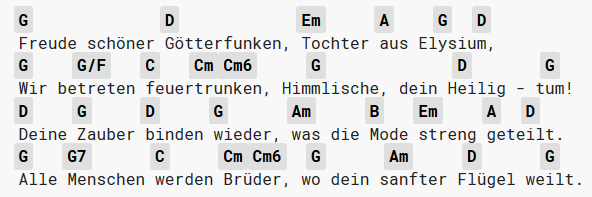
\includegraphics[scale=0.9]{images/ode_to_joy.png}
	\caption{Акорден запис}
	\label{fig:akordi}
\end{figure}

\subsection{Аспекти на податочна репрезентација за моделите за машинско учење}

Начинот на кој се трансформира изворниот формат на музиката во формат погоден за моделите за машинско учење драстично влијае на генерациските перформанси на моделот. Мали промени во податочната репрезентација може да доведат до израз различни музички особености во процесот на генерализација и генерирање на музика. Во продолженије ќе разгледам некои од клучните аспекти на податочната репрезентација.

\subsubsection{Репрезентација на времето}

Времето може да одлучиме да го претставиме како основен елемент на податочната репрезентација, т.е. да ја поделиме музиката во временски исечоци, или да го вградиме како параметар на основните елементи на музичката секвенца, слично како што е тоа направено во MIDI датотеките. Првиот случај е многу почест, скоро исклучиво искористен во минатите трудови (ЦИТИРАЈ СИТЕ ШТО СЕ СО ПИАНО ЛЕНТИ И ДРУГО ШТО НАЈДЕШ). Предностите му се што е едноставен за креирање на податочен енкодинг и недвосмислена претстава на времето и поедноставен приказ на акорди и полифонија. Недостатокот е реткоста (sparsity) на добиените примероци и честото повторување на идентични елементи во секвенците, на што драстично влијае грануларноста (резолуцијата). Можни се поделби на времето според реално време (пр. милисекунди) (ЦИТИРАЈ СИТЕ ШТО СЕ СО ПИАНО ЛЕНТИ И ДРУГО ШТО НАЈДЕШ), кадешто обично резолуцијата е порамнета со одредено нотно времетраење, и поделба на времето по времетраење на нотите (или метричка поделба) \cite{Walder2016}. Поделбата по ноти има потенцијал за побалансирано податочно множество, меѓутоа за влече со себе големи ограничувања за структурата на песните (нпр. промена на темпо може да резултира во големи дисторзии во добиената репрезентација).
Претставање на времето како дел од елементите на музичката секвенца пружа многу голема флексибилност, меѓутоа има доста недостатоци како нпр: нема ефикасен начен за енкодирање на времето во елементите, тоа ја експлодира големината на лексиконот на податочното множество, е многу комплексно да се енкодираат промени во тековно отсвирени ноти, пример при промена на акорди, каде дел од нотите би останале активни, дел би престанале да се свират, а нови би биле активирани. Се ова влијае драстично на перформансите на хипотетички модел за генерирање на музика.

\subsubsection{Краеви на нотите}

При репрезентација на музиката со временски исечоци не постои не можеме да разликуваме помеѓу две исти ноти отсвирени во два последователни исечоци и една нота со времетраење еднаква на сумата од времетраењето на двете поединечни ноти. Проблемот може да се пристапи на 3 начини:
\begin{itemize}
    \item Да се игнорира.
    \item Да се дуплира резолуцијата/грануларноста на податочната репрезентација од најмалото времетраење кое го има во податоците (или произволно одредено времетраење) со што ќе се додаде симбол за крај на ноти кој би се користел во секој друг временски чекор.
    \item Да се дуплира лексиконот на влезното множество, со што за секоја нота ќе има 2 симболи, еден за почеток еден за продолжување на нотата.
\end{itemize}
Вториот и третиот пристап го решаваат проблемот, меѓутоа ја дуплираат пресметковната комплексност на проблемот на учење и генерирање на музика.

\subsubsection{Резолуција}

При репрезентација на музиката со временски исечоци клучен фактор кој влијае на перформансите е резолуцијата/грануларноста на репрезентацијата. Поголема грануларност овозможува репрезентирање на по интересни, брзи, комплексни мелодии, меѓутоа резултира во поголеми мемориски побарувања на моделот за учење на таквите музички секвенци. Додатно зголемување на грануларноста резултира и во поголем број на празни елементи, и нотите со подолго времетраење ќе се повторуваат. Најчест пристап е да се одбере грануларност ендаква на најмалото времетраење на нота во податочното множество, меѓуто тоа не е секогаш така. Доколку релативно мал дел од елементите во податочното множество го имаат најмалото времетраење, може да се скоконе кон поголемо времетрање со цел поедноставување на проблемот.

\subsection{Пиано лента}

Пиано лента е најчесто искористената податолна репрезентација за работење со музика со модели за машинско учење (ЦИТИРАЈ ИСКОРИСТЕНА ПИАНОЛЕНТА). Музиката е поеделена на временски чекори, кадешто секој елемент претставува временски пресек со должина од дел од цела нота, или дел од секунда. Секој временски чекор ги претставува тековно исвирените ноти. Најчесто е бинарен вектор, кадешто секој елемент од векторот претставува одредена нота, според апсолутната вредност на висина на тонот (најчесто преку користење на pitch вредностите на нотите од MIDI стандардот), при што ненулта вредност означува дека таа нота се свири во моментот. Во одредени варијанти векторот може да биде целоброен, при што ненултите вредности опишуваат некоја особина на отсвирената нота како гласност или интензитет. Инспирирана е од старите пиано ленти од перфорирана хартија користени во само-свиречки пиана или метални ленти од музички кутии.
(СЛИКА ОД СТАРА ПИАНО ЛЕНТА, РЕАЛНА)
(СЛИКА ОД ПИАНО ЛЕНТА, The x axis represents time and the y axis the pitch.)

\subsection{Дистрибуирани репрезентации / круг на петинки}

Освен преку апсолутна вредност на висина на тон, нотите може да се репрезентираат и со семантички збогатена комплексна форма. Во трудот \cite{Mozer1994} авторот користи комбинација од основна фрекфенција, хроматска класа и позиција во "круг од петинки" за претставување на нотите, додека во трудот \cite{Biles1994} авторот ги репрезентира нотите во однос на акордите што тие ги придржуваат. Акордите се дел од една секвенца а нотите од друга, пропратна секвенца. Нотите имаат 14 можни висини од MIDI стандардот, а висината на тонот се одредува според придружниот акорд.
(ПОТЕНЦИЈАЛНО ОТСТРАНИ)

\section{Предпроцесирање}

По одбирање на податочно множество и репрезентација на истото за потребите на моделот за машинско учење може да се применат оптимизации постапки врз податоците пред извршување на алгоритамо за машинско учење.
Филтрирање на податочно множество, т.е. отстранување на песни, користејќи одреден сет на критериуми за конзистентност може да помогне во подобрување на перформансите на системот. Критериумите можат да бидант нпр:
\begin{itemize}
    \item Сите песни да се напишани во конкретен клуч.
    \item Сите песни да се во одредена метрика.
    \item Сите песни да се во одреден опстег на темпо.
    \item Да нема промена на метрика во песната.
    \item Песните да се комплетни и да нема оштетени или тешки за парсирање или двосмислени елементи.
    \item Нотите да припаѓаат само во одреден тонален распон.
\end{itemize}
Додатно филтрирање може да биде извршено и во рамките на песните. Елементи од изворните податоци кои не носат експлицитно музички податоци обично може да се отстранат без последици. Одредени музички елементи кои вршат модификации на музичките елементи може да се отстранат со последицата дека се губат одредени нуанси на отсвирената музика. Информацијата за интензитет/гласност на отсвирена нота може истотака да се отстрани со загува на нуанса. Доколку има ноти со помало времетраење од времетрање кое ќе го избереме за минимално тогаш пократките може да се отстранат или продолжат. Доколку одлучиме да работиме во ограничен тонален распон, нотите кои спаѓаат надвор од распонот може да ги отстраниме или поместиме внатре во тоналниот распон.

\subsection{Транспозиција}

Транспозиција е техника за поместување на множество од ноти за одреден број на полутонови нагоре или надоле со константен интервал. Може да се искористи врз колекција од песни за збогатување на податочното множество. Поместувајки ги сите мелодиски линии во податочното множество во сите можни позиции во тоналниот опсег му овозможува тонална инваријанса (транслациона инваријанса во друг контекст) на моделот за машинско учење и придонесува кон намалување на реткоста (sparsity) на тренинг податоците. Транспозицијата може да се изврши на сите песни кон еден заеднчики основен клуч (пр. \cite{Sturm2016,Tikhonov2017}) или на сите песни кон повеќе (потенцијално сите можни) основни клучеви (пр. \cite{Yang2017,Bretan2016}).

\chapter{Алатки}
\label{ch:alatki}

Во продолжени ќе дадам краток опис на алатките кои ги искористив за изработка на трудот.

\section{Keras}

Керас е библиотека за работа со невронски мрежи на високо ниво. Напишана е во Python и може да работи користејќи една од трите најпопуларни библиотеки за машинско учење на ниско ниво: ensorFlow, CNTK или Theano. Приоритет на библиотеката е овозможување на брзо и едноставно креирање на прототипи со користење на машинско учење така што ќе биде едноставна за разбирање и користење прво од човечка страна потоа од машинска. Паралелно процесирачките способности може да се користат на процесор или графичка картичка. Библиотеката е екстремно модуларна, скоро сите елементи кои што се конфигурабилни во невронските мрежи се модули и лесно може да се менуваат. Истите модули се отворени и може да бида проширени или заменети од корисничка страна.

\section{Music21}

Music21 е Python библиотека за музикологија, развиена на MIT. Намета е да овозможни лесна и детална анализа на музички композиции во симболична форма. Покрај разни музички анализи на постоечка музика, овозможува и модифицирање на истите, како и програматско креирање на музика и музички примероци. Поддржува низа на формати, од кои најзначајни се MIDI и musicxml. Покрај тоа содржи и повеќе колекции на класична музика во јавен домен кои може да се искористат за анализа или за тренирање на моделот за генерирање музика. 

\section{pypianoroll}

Pypianoroll е Python библиотека за работа со пиано лента записи. Подржува работа со записи со една лента или повеќе ленти, како и можности за транспозиција на постоечки пиано ленти. Овозможува и конверзија на MIDI датотеки во пиано лента и обрано, како и графичка визуелизација на пиано лентите.

\chapter{Студија на случај}
\label{ch:studija}

\section{Податочно множество}

Најдостапен и најлесен за комјутерска обработка извор на симболична музука претставуваат МИДИ датотеките. Во иницијалните фази на изработка користев мало податочно множество коешто го изградив од GuitarPro датотеки рачно избрани од http://ultimate-guitar.com. Датотеките преставуваат кориснички генерирана репрезентација на музиката, примарно наменети за учење. Бидејќи системот за репродукција на звук за GuitarPro датотеките е базиран на MIDI стандардот, можев лесно да ги конвертирам во MIDI датотеки. Финалниот чекор за подготовка на податоците е трансформација во пиано лента репрезентација. За жал процесот резултираше во неквалитетна конверзија, песните во финалната форма има многу аномалии, неправилности и изгубена смисла на одредени елементи. Се појавија многу тонови со времетраење од 0 рамки, како и тонови со времетраење од десетици секунди. Исто така се појавија истровремено свирење на 10 и повеќе тонови на гитара, што е невозможно со стандардна гитара. Добар дел од проблемите следат од тоа што датотеките се кориснички генерирани што не гарантира квалитет, како и од алатките за конверзија. Затоа одлучива да ја напуштам оригиналната замисла и да користам готово податочно множество.

\subsection{Лахк (Lahk) MIDI}

Лахк MIDI податочното множество се состои од 176.581 уникатни MIDI датотеки, соберени од страна Рафел за целите на неговоит труд \cite{Raffel2016} во кој покажува систем за пребарување и споредување на секвенци, или исечоци, од MIDI датотеки. Дел од овие множеството, наречен LMD-Matched, се состои од 45.129 датотеки спарени со соодвенти метаподатоци од датабазата MillionSongs, што овозможува пребарување, групирање и селекција по одредени критериуми како жанр, автор, стил, темпо и сл. 
Врз основа на LMD-Matched податочното множество, Донг за потребите на трудот \cite{Dong2017} го имат конвертирано целото податочно множество во пиано лентал. На веб страната на која е прикажан нивниот труд се достпни повеќе верзии од множеството:

\begin{itemize}
    \item LPD-Cleansed - Претставува прочистена верзија на податочното множество според следните критериуми: отстранети песни кои не се со 4/4 ритам, отстранети песни со повеќе од една промена на ритам, остранети песни каде што првиот такт не почнува од нулти момент, задржани песните кои што со наголема сигурност се спарени со ставка од MillionSongs датабазата.
    \item LPD-5 - Сите можни инстанци на инструменти во MIDI датотеките се групирани во следните 5 категории: тапани, пиано, гитара, бас и жичана секција; според MIDI програмскиот број на инструментот. Неголем дел од инструментите кои не припаѓаат на ниту една од овие категории се групирани во жичаната секција, со исклучок на синтисајзер, перкусии и звучни ефекти.
    \item LPD-17 - Слично на претходното множество со тоа што инструментите се групирани во 17 категории: тапани, пиано, хроматски перкусии, оргуља, гитара, бас, жичана секција, ансамбл, метални дувачки инструменти, дрвени дувачки, писка, главен синтисајзер, придружба синтисајзер, етнички инструменти, перкусии и звучни ефекти.
\end{itemize}

LPD-5 податочното множество се покажа како одлична појдовна точка за изградба на помало податочно множество за експериментите, бидејќи содржи песни со константен 4/4 ритам. Меѓутоа не е доволно добро за употреба без модификација. Не сите песни ги имаат сите инструменти, а некои песни имаат повеќе инструменти групирани во една трака, така да потребна е додатна обработка и селекција за да се добие квалитетно податочно множество.

\section{Податочна репрезентација}

Песните во LPD-5 податочното множество се во пиано лента репрезентација, каде што времето е поделено така што една рамка од лентата претставува 1/24 од еден такт. Една рамка се содржи од 128 целобројни вредности, по една за секоја од можните ноти или звуци опишани со MIDI стандардот, при што вредноста го опипува интензитетот со кој се присутен звукот. Ваквиот вектор не е адекватен за учење на секвенци, бидејќи преставува решавање на 128 регресионони проблеми во паралела. Затоа првиот чекор во прилагодување на векторот претставува бинаризација, т.е. во секоја рамка секоја ненулта вредност се заменува со единица. Во обратна насока, при дебинаризација на векторот, единиците ги заменувам со рачно одредена вредност за интензитет, 2/3 од максималната вреднос. На овој начин се губи експресивност и нуанса, меѓутоа драстично се олеснува проблемот на учење на секвенци. 
По иницијални експерименти каде што тренирав модел да учи секвенци од тн. "multi-hot" вектори (бинарни вектори каде што повеќе вредности може да бидат активни истовремено), како што е бинаризираната варијанта на пиано ленти, дојдов до заклучок дека ваквите секвенци претставуваат тежок проблем за учење за моделите коишто сакав да ги искористам. Учење на 128 паралелни проблеми резултираше во многу ретки активации на излезниот слој, а во рамките кадешто се појавија повеќе активации, комбинациите на ноти често беа бесислени. Поради тоа одлучив да изградам лексикон од сите можни комбинации на ноти, и да ги користам елементите од лексиконот како влезе во моделот за учење. Трансформацијата ја извршив така што 128 елементниот вектор го сметам како 128 битна бинарна репрезентација на цел број. Лексиконот го изградив од ваквите целобројни репрезентации со додатни симобили за почеток и крај на песна/секвенца. Лексиконот потоа го индексирав и секој елемент доаѓа на влез на моделот во "one-hot" или 1-n бинарен вектор, во кој што сите вредности се нула, само вредноста со ист индекс како елементот од лексиконот е единица.

\section{Селекција на песни}

Датотеките од податочното множество содржат 5 траки кои ги преставуваат инструментите: тапани, пиано, гитара, бас и жичана секција. Меѓутоа не сите датотеки имаат податоци во сите траки, т.е. не е извршена претходно филтрирање на песните така што сите песни да ги имаат сите инструменти. Додатно бидејќи во жичана секција се групирана многу инструменти, што често може да доведе и до групирање на повеќе траки од изворната датотека во една, одлучив да ги филтрирам сите датотеки што содржат податоци на таа трака. Додатно голем број на песни не содржат пиано трака, а бидејки фокусот ми беше на рок песни коишто најчесто немаат пиано делови, ги исфилтрирав и пените што содржат пиано. Останатите песни ги филтрирав така да пиано лентите за траките тапани, гитара и бас гитара се целосно исполнети. Од добиеното подмножество со случајна селекција избрав 500 песни, од коишто поголем дел природно се погодија од рок, поп-рок и метал жанр. Од ова подмножество креирав MIDI датотеки со користење на pypianoroll библиотеката. Потоа со рачна инспекција на песните една по една избрав (ФИНАЛНА БРОЈКА НА ПЕСНИ) според субјективна процена за квалитетот на добиената датотека, познавање на песната, жанровска припадност и релативна едноставност на песната.

\section{Транскрипција на песните}

За збогатување на податочното множество и гарантирање на транслациона инваријанса на мелодиските линии искорив постапка на музичка транскрипција. Прво ги одредив најнискиот и највисокиот тон присутен во избраното податочно множество. Потоа за секоја од песните извришив транскрипција надолу за толку полутонови колку што има од најнискиот тон во податочното множество и најнискиот тон во самата песна, и нагоре за толку полутонови колку што има помеѓу највисокиот тон во податочното множество и највисокиот тон во поесната. Ваквата стратегија резултира во разлилен број на транскрипција по песна, зависно од колку голем е тоналниот опсег на песната, што значи некои песни се поприсутни во резултантното транскрибирано податочно множество, а некои помалку присутни; но и во најголем можен број на транскрипции. Транскрипцијата ја извршив само на траките за гитара и бас, бидејќи нема смисла за тапани, таму миди тоновите не претставуваат ноти на ист начин како кај останатите инструменти, туку тип на удар и инструмент за удар.

(ЦИТИРАЈ ТРУД ЗА ТРАНСКРИПЦИЈА), (БРОЈКА НА ТРАНСКРИБИРАНИ ПЕСНИ)

\section{Упростување на проблемот}

Вака добвиеното потадочно множество претставуше алгоритамски и технички проблеми за процесот на учење. Најлош случај се јавува кај гитарата. Теоретски во најлош случај можни се 128*127*126*125*124*123=3*10e13 комбинации на ноти според MIDI стандардот, или според физичките ограничувања на гитара 24*6=191.102.976 можни комбинации на ноти. Во еден од експериментите со 50 песни со целосна транскрипција не беше возможно извршивање на моделот бидејки лексиконот напросто експлодираше во големина, па не беше возможно извршување на моделот во меморија, на систем со NVIDIA Tesla K80 со 24GB меморија што е горниот лимит на достапен хардвер. Моделот имаше вкуно (ЦИТИРАЈ БРОЈ НА ВЕЛЗНИ ПАРАМЕТРИ) велзни параметри. Покрај тоа што невозможно за изршување, претпоставувам дека би се разредило, т.е. би се разделиле активациите на премногу елементи, и би било потешко за анализа и дебагирање. Затоа одлучив да изврша консолидација на податочното множество и негово упростување.

\subsection{Поедноставување на акордите, намалување на бројот на можни комбинации}

По пребројување на инстанците од сите комобнации на ноти низ податочното множество увидов дека сите категории на акорди не се подеднакво застапени. Најчесто се појавуваат дурски и молски триади, и рок (познати и како "power") акорди како и поединечни ноти. Во (ЛИНК ДО ТАБЕЛА) може да се види честотата на појавување на акордите по категории. Одлучив да ги заменам акордите чии категории не се појавуваат со повеќе од 1\% со основната нота на акордот, а останатите акорди да ги упростам до 3 нотни верзии. Задржани се акордите од следните категории: (ЛИСТА ОД ФОРТЕ КЛАСИ). Оваа трансформација сметам дека нема премногу да го наруши карактерот на музиката, а сепак ќе ја намали пресметковната комплексност во граници на практична изведба.

(ТАБЕЛА НА ПОЈАВУВАЊА НА ТИПОВИ НА АКОРДИ)

\section{Архитектура за учење}

Архитектурата е имплементирана со користење на Keras библиотеката за длабоко учење, па така некои термини и имиња доаѓаат од терминологијата на библиотеката.
Моделот за учење се состои 3 подмодели, по еден за секој од инструментите. Моделите меѓусебе се идентични, претставени со (ЛИНК ДО ДИЈАГРАМ НА МОДЕЛ). Една влезна рамка за секој од моделите се сотоид од 3 вектори кои ја претставуваат тековно исвирената комбинација на ноти за конкретниот инструмент во временскиот момент кој го претставува рамката. Моделите започнуваат со 3 блока, еден блок кој на влез прима N временски рамки од тековниот временски момент наназад, еден блок на влез ја примат тековната временска рамка, а последниот модел прима N временски рамки нанапред.

Секој од блоковите има излез во тн. ембединг блок (невронска подмрежа) која претставува тесно грло, има помал број на јазлик од претходниот влезен слој, чија задача е да изверши компресија на податоците, и функционира слично на аутоенкодер архитектурата. Ваквите слоеви се искористени претходно во учење на секвенци од зборови (ЦИТИРАЈ ТРУДОВИ ЗА WordEmbeddings) и покрај тоа што прават пресметковно олеснување, учат и веројатности за истровремено појавување на елементите.

По ембединг слојот следуваат 2 LSTM подмрежи и една целосно поврзана мрежа. Излезот од ембединг блоковите одговорни за секвенците од временски рамки оди во LSTM подрежите, додека излезот од ембединг блокот за тековната рамка оди во целосно поврзаната мрежа. LSTM мрежите ги учат временските зависности за соодветниот инструмент врз основа на временските рамки од минатото и иднината, додека целосно поврзаната мрежа ги учи зависностите на тековно исвиреното од соодветниот инструмент и останатите инструменти во даден временски момент. 

Излезите од LSTM мрежите и целосноповрзаната мрежа ги комбинирам во еден велзен вектор за финална целосно поврзана мрежа, чија задача е да ја учи, и подоцна предвиди, тековно отсвирената комбинација ноти за соодветионит инструмент.

\subsection{Ембединг на акорди}

Ембединг блоковите се изградени од цеслосно поврзана невронска мрежа со еден слој од 256 јазли. Влезната димензија на слојот е еднаква на големината на лексиконот, а излезот е реално вредностен вектор од 256 елементи.

(ДИЈАГРАМ ОД СЛОЈ)

\subsection{Основен ЛСТМ мрежа за секвенци}

Двете LSTM мрежи се составени од два слоја по 256 LSTM јазли. Влезната димензија е еднаква на излезот од ембединг слојот помножен со бројот на временски чекори кој се гледа наназад, или нанапред (32), познат како lookback, а излезот е реалновредностен вектор со 256 елементи, со активациска функција тангенс хуперболикус. Излезите ги претставуваат предвидувањата за тековниот чекор врз основа на временскиот сегмент што го надгледува конкретниот блок. Бројот на временски чекори кој се гледа наназад и или нанапред е всушност Back Propagation Through Time, или поточно неговата скратена варијанта Truncated Back Propagation, во Keras одредена со големината на субсеквенца од временски чекори коишто и се даваат на LSTM подмрежата во одреден момент. 
(ДИЈАГРАМ ОД СЛОЈ)

\subsection{Целосно поврзана мрежа за тековната временска рамка}

Овој блок е изграден од еден целосно поврзан слој од 256 јазли. Влезната димезија е еднаква со големината на излезот од ембеинг слојот, а излезот е реално вредностен вектор од 256 елементи, со ReLU (Rectified Linear Unit) активација.

(ДИЈАГРАМ ОД СЛОЈ)

\subsection{Блок за предвиување}

Излезите/предвидувањата од двете LSTM мрежи и целосно поврзаната мрежи ги спојувам во еден поголем вектор кој служи како влез во финалниот блок за предвидување. Овој блок е составен од целосно поврзан слој од број на јазли еднаков на големината на лексиконот. Влезната димензија еднаква на збирот од излезни димензии од претходните блокови за предвидување, а излезот е бинарен вектор со димензија ендаква на големината на лексиконот, со softmax активација. Излезот од овој блок го дава конечното предвидување за вредноста отсвирена од конкретниот инструмент во тековниот временски чекор.

(ДИЈАГРАМ ОД СЛОЈ)

\section{Тренрање на моделот}



\section{Алгоритам за генерирање на песни}

Генерирање на песните го вршам со Псеудо-Гибсова техника за вадење на примероци од веројатносна дистрибуција, заедно со ситем за паралелно ажурирање на вредности (ЦИТИРАЈ PARALLEL GIBBS). Генерирањето започнува со симболот за почеток и трае до предвидување на симбол за крај или до максимална зададена должина на секвенца. Процесот на генерирање е итеративен, т.е. секој претходно предвиден временски чекор влијае на следното предвидување. Техниката предвидува употреба на параметар температура, кој што воведува стохастичност во процесот. Искористив почетна вредност од 1.5 и минимална вредност од 1.0. Колку поголема вредноста има температурата толку е понепредвидлив изборот на следниот елемент во процесот на предвидување, а колку е понизок процесот станува се по-детерминистички. 

min_temperature = temperature
temperature = 1.5
    
 temperature = max(min_temperature, temperature * 0.9992)

\cite{Hadjeres2016} ALGORITHM Generation in dependency networks is performed using the pseudo-Gibbs sampling procedure. This Markov Chain Monte Carlo (MCMC) algorithm is described in Alg.1. It is similar to the classical Gibbs sampling procedure (Geman & Geman, 1984) on the difference that the conditional dis- tributions are potentially incompatible (Chen & Ip, 2015). This means that the conditional distributions of Eq. (2) do not necessarily comes from a joint distribution p(V) and that the theoretical guarantees that the MCMC converges to this stationary joint distribution vanish. We experimen- tally verified that it was indeed the case by checking that the Markov Chain of Alg.1 violatesKolmogorov’s criterion (Kelly, 2011): it is thus not reversible and cannot converge to a joint distribution whose conditional distributions match the ones used for sampling. However, this Markov chain converges to another station- ary distribution and applications on real data demonstrated that this method yielded accurate joint probabilities, espe- cially when the inconsistent probability distributions are learned from data (Heckerman et al., 2000). Furthermore, nonreversible MCMC algorithms can in particular cases be better at sampling that reversible Markov Chains (Vucelja, 2014). 2.3.2. We emphasize on this section the importance of our partic- ular choice of data representation with respect to our sam- pling procedure. The fact that we obtain great results using pseudo-Gibbs sampling relies exclusively on our choice to integrate the hold symbol into the list of notes. Indeed, Gibbs sampling fails to sample the true joint dis-
tribution p(V|M, θ) when variables are highly correlated, creating isolated regions of high probability states in which theMCMCchain can be trapped. However, many data rep- resentations used in music modeling such as
• the piano-roll representation,
• the couple (pitch, articulation) representation where articulation is a Boolean value indicating whether or not the note is played or held,
tend to make the musical data suffer from this drawback.
As an example, in the piano-roll representation, a long note is represented as the repetition of the same value over many variables. In order to only change its pitch, one needs to change simultaneously a large number of variables (which is exponentially rare) while this is achievable with only one variable change with our representation.

\section{Анализа на резултати}

\chapter{Заклучок}
\label{ch:zaklucok}